\section{Implementation}

Currently we have implemented the interpolant algorithms in Haskell. We have tested
the Haskell implementation with the examples provided in Kapur's paper.

\begin{figure}[h]
  \centering
  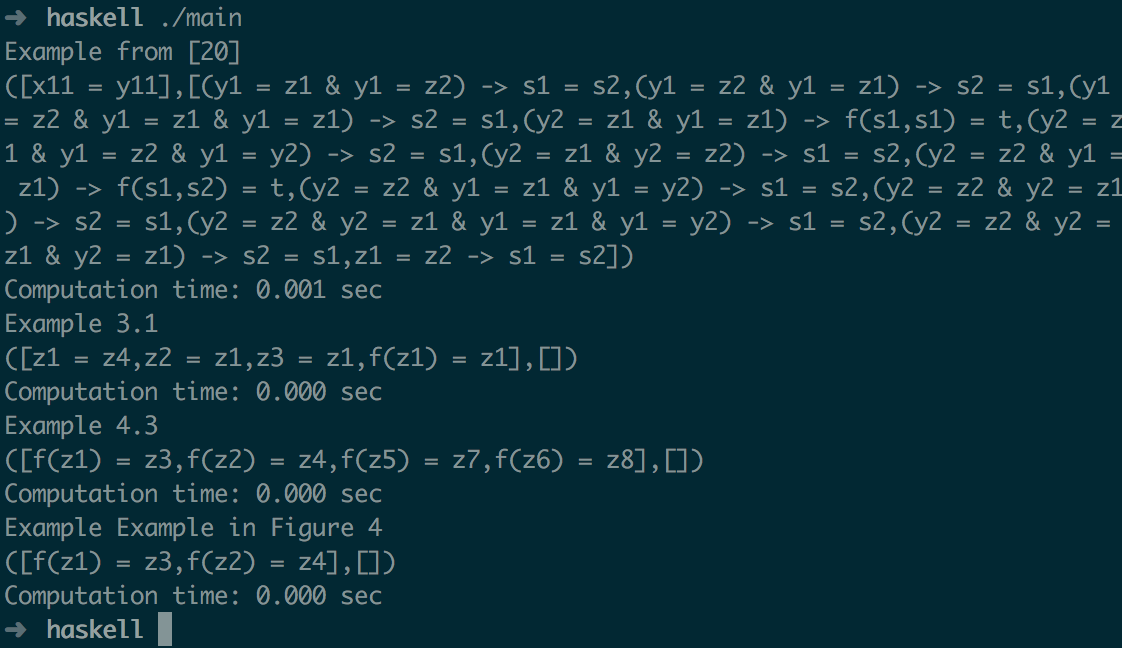
\includegraphics[width=8cm]{eufPerformance}
  \caption{Timming of Haskell program to compute EUF interpolants}
\end{figure}

The implementation of the implicational closure and fast congruence closure
are efficient implementations in C++. We have tested the software with
several automated examples with around 10000 terms. The testing consisted
in checking if the congruence closure was computed as expected, i.e. we checked
every possible pair of terms and check if they are in the congruence
relation iff their successors are already in the congruence relation.

To measure performance we automated several examples. The results of running
time of the algorithm are shown below:

\begin{figure}[h]
  \centering
  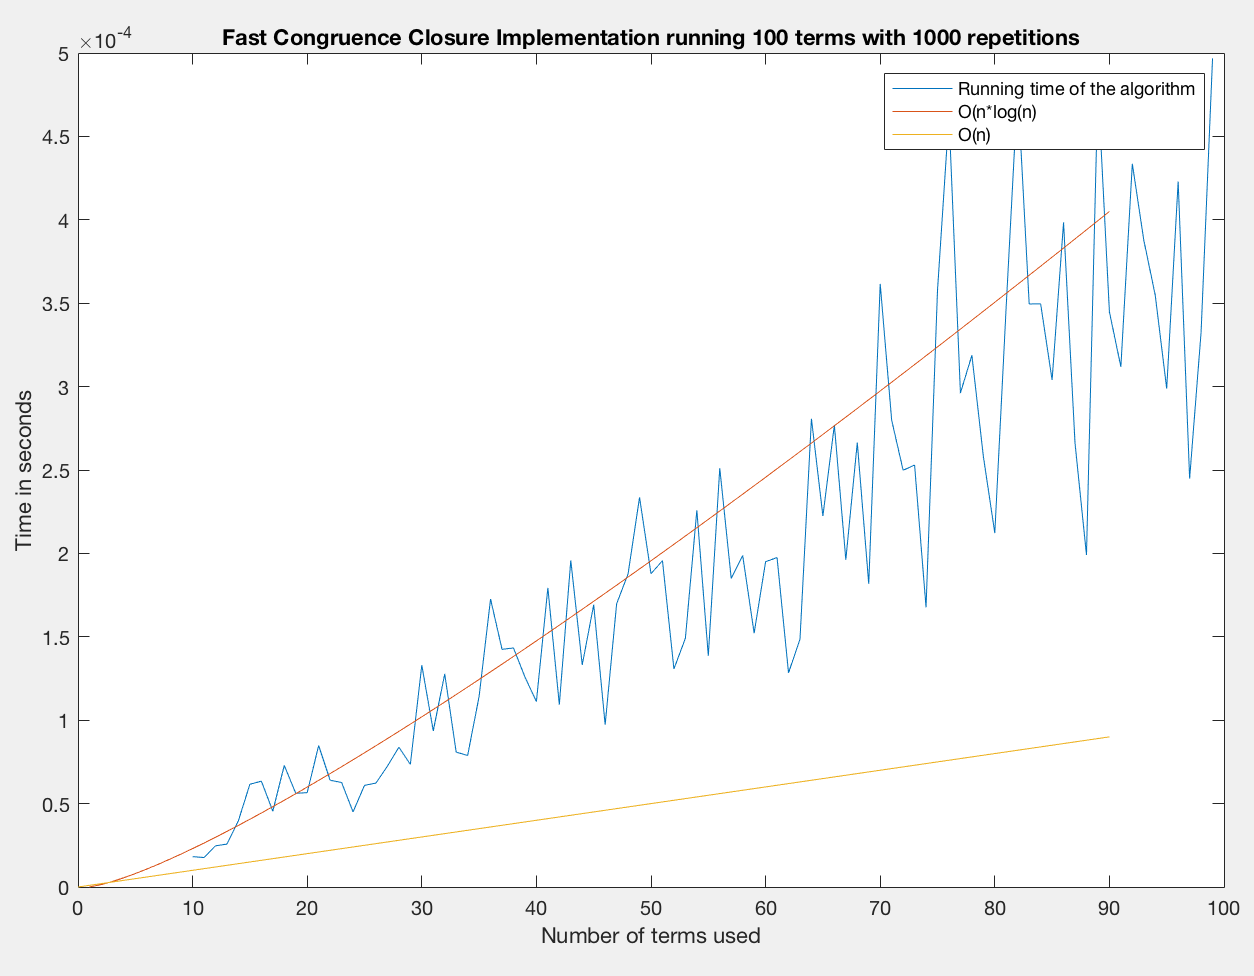
\includegraphics[width=8cm]{100_1000rep}
  \caption{Comparison of running time of the fast congruence closure implementation with
    $\bigO{n \log n}$ and $\bigO{n}$ functions executing 100 terms and doing 1000 repetitions.}
\end{figure}
\begin{figure}[h]
  \centering
  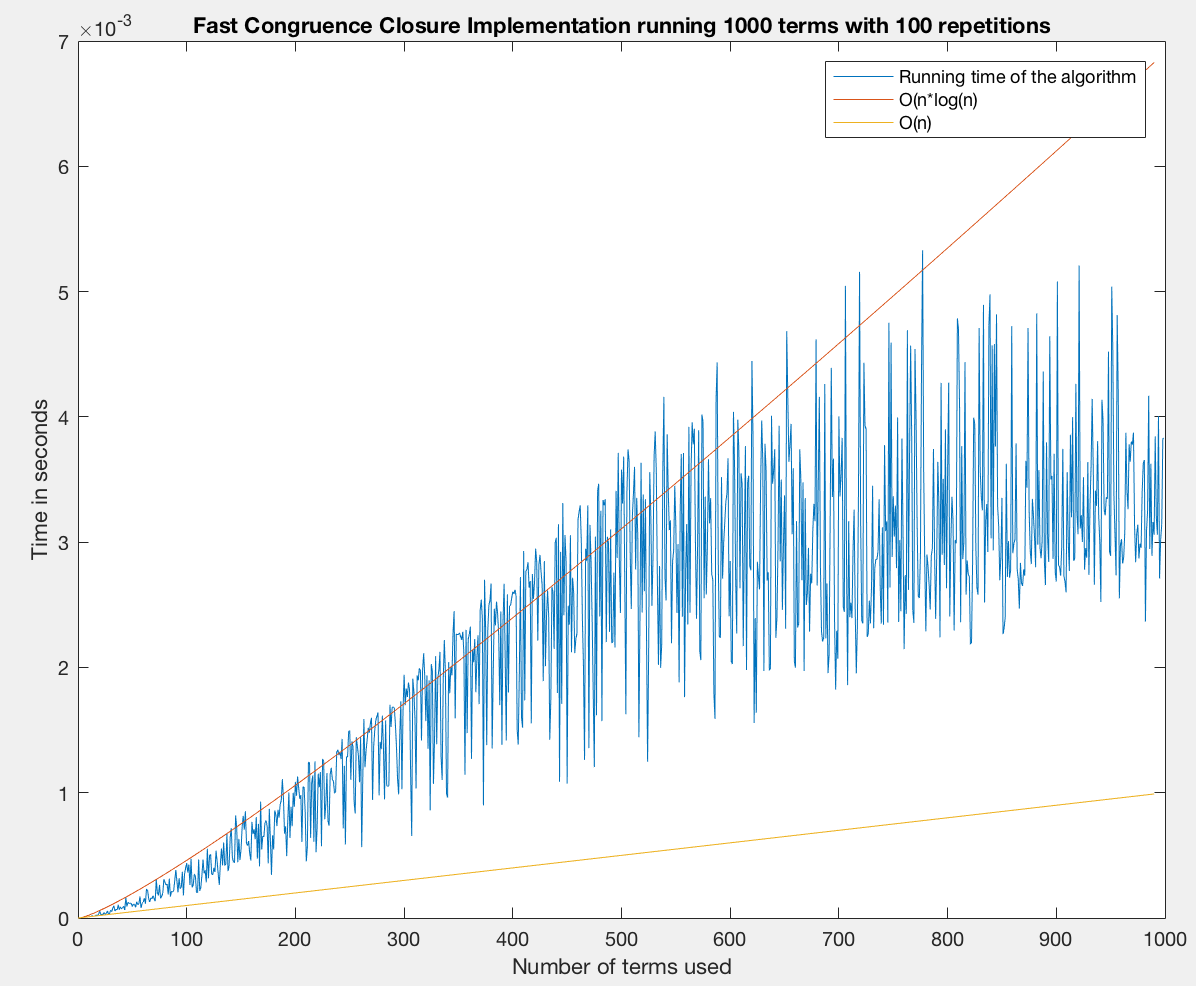
\includegraphics[width=8cm]{1000_100rep}
  \caption{Comparison of running time of the fast congruence closure implementation with
    $\bigO{n \log n}$ and $\bigO{n}$ functions executing 1000 terms and doing 100 repetitions.}
\end{figure}
\begin{figure}[h]
  \centering
  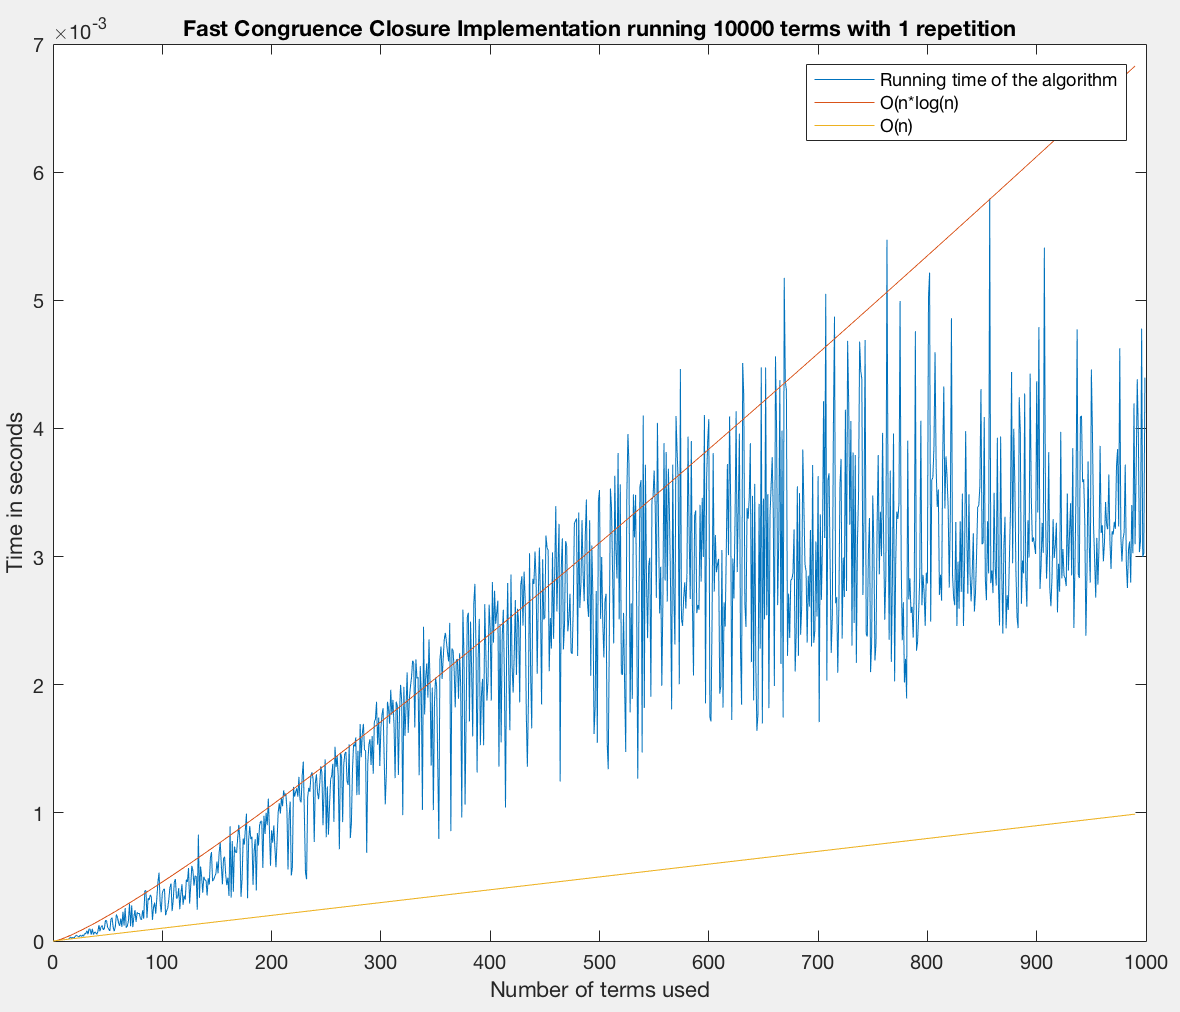
\includegraphics[width=8cm]{10000_1rep}
  \caption{Comparison of running time of the fast congruence closure implementation with
    $\bigO{n \log n}$ and $\bigO{n}$ functions executing 10000 terms and doing 1 repetitions.}
\end{figure}
